\documentclass{article}\usepackage[]{graphicx}\usepackage[]{color}
%% maxwidth is the original width if it is less than linewidth
%% otherwise use linewidth (to make sure the graphics do not exceed the margin)
\makeatletter
\def\maxwidth{ %
  \ifdim\Gin@nat@width>\linewidth
    \linewidth
  \else
    \Gin@nat@width
  \fi
}
\makeatother

\definecolor{fgcolor}{rgb}{0.345, 0.345, 0.345}
\newcommand{\hlnum}[1]{\textcolor[rgb]{0.686,0.059,0.569}{#1}}%
\newcommand{\hlstr}[1]{\textcolor[rgb]{0.192,0.494,0.8}{#1}}%
\newcommand{\hlcom}[1]{\textcolor[rgb]{0.678,0.584,0.686}{\textit{#1}}}%
\newcommand{\hlopt}[1]{\textcolor[rgb]{0,0,0}{#1}}%
\newcommand{\hlstd}[1]{\textcolor[rgb]{0.345,0.345,0.345}{#1}}%
\newcommand{\hlkwa}[1]{\textcolor[rgb]{0.161,0.373,0.58}{\textbf{#1}}}%
\newcommand{\hlkwb}[1]{\textcolor[rgb]{0.69,0.353,0.396}{#1}}%
\newcommand{\hlkwc}[1]{\textcolor[rgb]{0.333,0.667,0.333}{#1}}%
\newcommand{\hlkwd}[1]{\textcolor[rgb]{0.737,0.353,0.396}{\textbf{#1}}}%

\usepackage{framed}
\makeatletter
\newenvironment{kframe}{%
 \def\at@end@of@kframe{}%
 \ifinner\ifhmode%
  \def\at@end@of@kframe{\end{minipage}}%
  \begin{minipage}{\columnwidth}%
 \fi\fi%
 \def\FrameCommand##1{\hskip\@totalleftmargin \hskip-\fboxsep
 \colorbox{shadecolor}{##1}\hskip-\fboxsep
     % There is no \\@totalrightmargin, so:
     \hskip-\linewidth \hskip-\@totalleftmargin \hskip\columnwidth}%
 \MakeFramed {\advance\hsize-\width
   \@totalleftmargin\z@ \linewidth\hsize
   \@setminipage}}%
 {\par\unskip\endMakeFramed%
 \at@end@of@kframe}
\makeatother

\definecolor{shadecolor}{rgb}{.97, .97, .97}
\definecolor{messagecolor}{rgb}{0, 0, 0}
\definecolor{warningcolor}{rgb}{1, 0, 1}
\definecolor{errorcolor}{rgb}{1, 0, 0}
\newenvironment{knitrout}{}{} % an empty environment to be redefined in TeX

\usepackage{alltt}

\title{Draft Outline -- SAS Report}
\author{2016 EA30 Students}
\IfFileExists{upquote.sty}{\usepackage{upquote}}{}
\begin{document}

\maketitle

\newpage
\tableofcontents
\newpage

\section{Introduction}

\subsection{Problem Statement}
This report aims to determine whether Biochemical Oxygen Demand (BOD) and water flow velocity are relevant to future research regarding the endangered Santa Ana sucker \emph{C. santaanae}. We collected water quality data from the Santa Ana River to answer the following questions: \emph{Do BOD levels vary in different sections of the river};\emph{do differing BOD levels affect correlate with the abundance of individuals?}; \emph{Do the water flow rates in different sections of the river correlate with sucker populations?} Because the part of the river we evaluated regularly receives discharge water from a water treatment facility, we believe that BOD levels will be POLYSEED, decreasing further from the discharge point. Where the BOD levels are lower, we expect there to be more fish. We also hypothesize that larger populations of the sucker will concentrate near high-flow sections. Through this experiment, we aim to inform Santa Ana sucker conservation efforts and hope to inform action by the nearby water treatment facility. 
=======


\subsection{Background (Literature Review)}
In general, fish have been known to be at risk of suffocation when exposed to dissolved oxygen (D.O.) levels below 2 mg/L for only short periods of time[2]. A 2012 U.S. Fish and Wildlife Service report on the recovery of the endangered fish noted that specific tolerances to dissolved oxygen have not been determined for  Santa Ana Sucker[1]. The 2012 FWS report also notes that constant water flows are important to the availability of coarse substrate which the Sucker needs to spawn offspring and hide from predators. According to Evans et al. (2005), temporary reduction of flows can significantly reduce the amount of habitat for suckers.[3] Just last month, the Center for Biological Diversity reported that ``by halting water releases critical to maintaining surface flows of the Santa Ana River, the Rapid Infiltration and Extraction (RIX) treatment plant is stranding and killing threatened fish.'' [4]

\subsection{Objectives}
We measured BOD levels and water flow velocity in different areas of the Santa Ana River and correlated those measurements with camera observations of Sucker abundance in both sample locations.
\begin{quote}
Our null hypotheses are H0: Water flow velocity and/or BOD levels do not significantly correlate with prevalence of the Santa Ana Sucker.
\end{quote}
\begin{quote}
Our alternative hypotheses are H1: Water flow velocity and/or BOD levels significantly correlate with prevalence of the Santa Ana Sucker.
\end{quote}
If we can reject one or both of our null hypotheses, we can conclude that the study of Biological Oxygen Demand (BOD) and water flow velocity are relevant to future conservation research for the endangered Santa Ana sucker \emph{C. santaanae}.

\section{Methods}

\subsection{Site Descrition}

We evaluated the Santa Ana River between... near Colton, California (Figure \ref{SAR_Image}). 

\begin{figure}
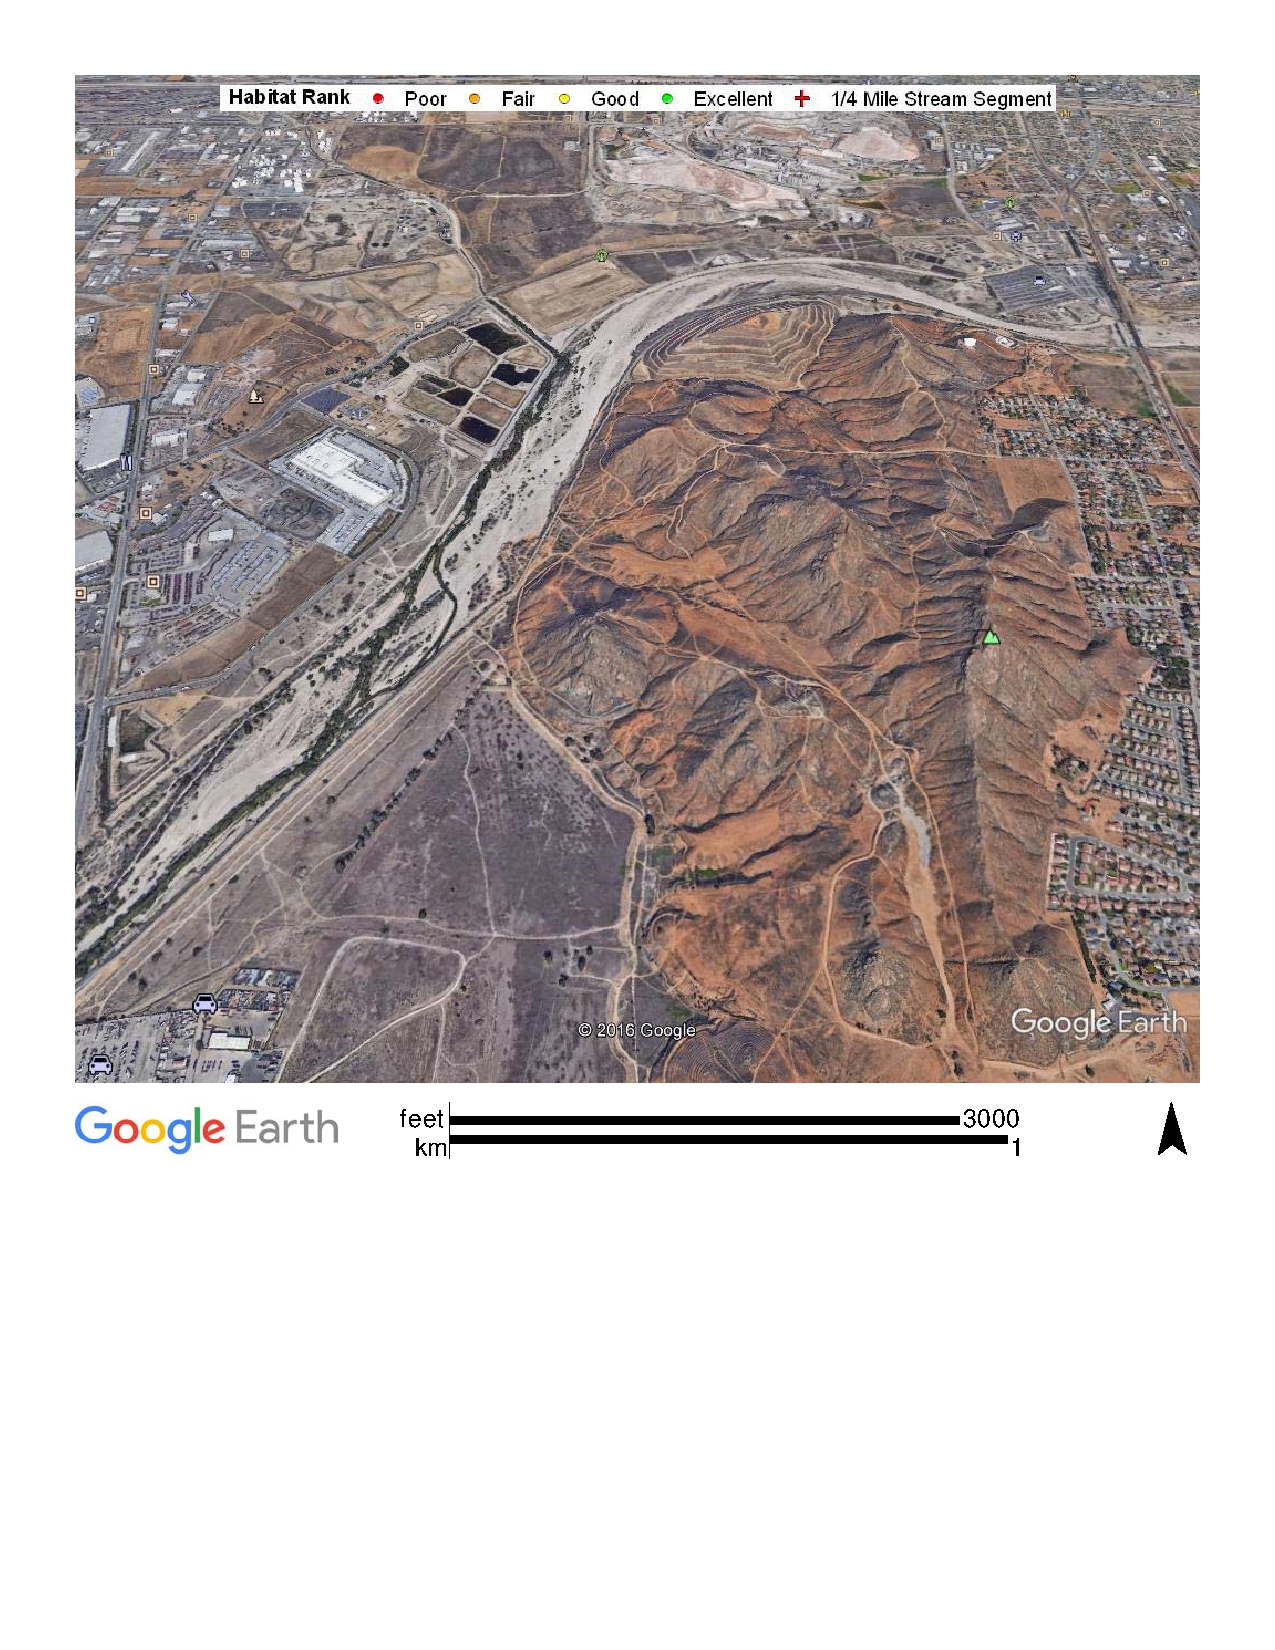
\includegraphics[width=1.00\textwidth]{Figures/SantaAna_SatelliteImage}
\caption{Google Earth --Example of a map. What's wrong with this image?}
\label{SAR_Image}
\end{figure}

\subsection{Field Methods}
\subsubsection*{5-Day Biochemical Oxygen Demand Test (BOD5)}
Approximately 1L of source river water was collected at each of two sites, one upstream location closer to the wastewater discharge facility, and one downstream location (fig. 1), which was transported to the laboratory for analysis within four hours.

\subsubsection*{Water Velocity Collection}
At each of the corresponding water sample collection sites, water velocity was also measured using a SonTek FlowTracker Handheld Advanced probe, which emits sonar waves at a certain depth in the water column, and based on the feedback (20 pings) gives a velocity reading. Ideally, multiple readings would be taken at each site, after the probe is placed on a flat section of the riverbed where water appears to be flowing in the same direction. 

\subsection{Laboratory Methods}
\subsubsection*{BOD5}
Ideally within the same day of collection, water samples are analyzed for initial dissolved oxygen content and prepared for 5-day incubation.  
\begin{itemize}
  \item Three different dilutions were used for each of two sites, with source water volumes of 25, 50, and 100 mL. 
  \item A seed suspension was prepared using PolySeed Seed Innoculum, and 4 mL of the solution was added to each 300 mL sample bottle. This solution was also used to create four seed blanks with seed volumes 15, 20, 25, and 30 mL.
  \item Nitrification inhibitor was created by dissolving 2.0 g allylthiourea (ATU, C4H8N2S) in 1 L distilled water. 0.3 mL of the ATU solution was added to each source water sample, as well as to all seeded samples. 
  \item A glucose-glutamic acid (GGA) solution was prepared by dissolving 150 mg each of dry glucose and glutamic acid in 1 L of distilled water, and was added to each of the four seed blanks, as well as the six source water samples. Three GGA blanks were also created with 6 mL of GGA solution in incubation bottles. 
  \item Dilution water was created using 1 mL each phosphate buffer (8.5 g KH2PO4, 21.75 g K2HPO4, 33.4 g Na2HPO*7H2O, and 1.7 g NH4Cl dissolved in 1 L distilled water), Magnesium sulfate solution (4.5 g MgSO4*7H2O dissolved in 200 mL distilled water), Calcium chloride solution (5.5 g CaCl2 dissolved in 200 mL distilled water), and Ferric chloride solution (0.05 g FeCl3*6H2O dissolved in 200 mL distilled water), and added to the six source water samples, four GGA blanks, and three seeded blanks. Three dilution water blanks were also created using the same procedure diluted to 300 mL.
\end{itemize}
Initial DO readings were to be taken on all blanks and samples using a Thermo Scientific DO Probe with auto-spinning functionality. The bottles were then incubated in a dark area for 5 days, and DO readings were again taken.    

\subsection{Statistical Methods}
\subsubsection*{Quality Control Checks}
Using the seed blanks, glucose-glutamic acid blanks, and dilution water blanks, quality control checks were performed prior to data collection. 
\begin{itemize}
  \item Minimum DO Depletion--Viable samples must have min. DO depletion of 2.0mg/L, and residual DO of at least 1.0mg/L.
  \item Glucose-Glutamic Acid Check--The resulting average BOD for the 3 GGA blanks (after correction for dilution and seeding) must be 198+/- 30.5mg/L.
  \item Dilution water check--DO uptake after incubation must not be more than 0.20mg/L and preferably not more than 0.10 (before seed corrections). 
  \subitem Dilution Water--If dilution water blank exceeds 0.20 mg/L, clearly identify samples in data.
  \item Seed control--Calculate Seed Control Factor (SCF) using [(D1-D2)*f], where
  \subitem D1= initial DO of seed control, mg/L
  \subitem D2= final DO after indubation, mg/L,
  \subitem f= (vol. seed in diluted sample)/(vol. seed in seed control)
\end{itemize}

\subsubsection*{BOD5}
BOD5 was calculated for viable samples according to Standard Methods for the Examination of Water and Wastewater, using the equation 
BOD5, mg/L= ((D1-D2)-(S)Vs)/P, where 
\subitem D1= initial DO, mg/L
\subitem D2= final DO after incubation, mg/L
\subitem S= oxygen uptake of seed, ∆DO/mL of seed suspension added per bottle
\subitem Vs= volume of seed in test bottle
\subitem P= decimal volumetric fraction of sample used.
The average of the resulting values for all viable samples was determined

\section{Results}
Analysis of the data using quality control parameters indicated that two source water samples met minimum DO depletion standards. Our BOD5 calculations of these data yielded the values:

\subitem Upstream BOD5= 22.069 mg/L 
\subitem Downstream BOD5= 27.3493 mg/L 

The average recorded water flow velocities were:
\subitem Upstream: 0.27 ft/sec
\subitem Downstream: 1.09 ft/sec 


\section{Discussion}
Due to the learning curve associated with performing a new experiment, procedural complications were encountered at several points in the experiment. As a result, initial DO content was not measured for the source water samples before incubation. We estimated a constant initial sample DO measurement using the DO of the seeded blanks. This decreased the accuracy of the BOD5 calculations, but gave a relative idea of the initial values. Inconsistent DO measuring methods also added to the inaccuracy of the final BOD5 results. Despite these procedural errors, our BOD5 measurements, 27.3493 mg/L at the downstream location and 22.069 mg/L at the upstream location, did reach quality control parameters.


It should also be noted that the water velocity averages were derived from a small sample size; three readings in total were taken, two from the downstream location and one from the upstream.


\section{Conclusion and Recommendations}
Future study of dissolved oxygen levels and water velocity in the Santa Ana River should correlate with recent Fish and Wildlife Service electroshock population data. Though we do not have access to this data, we do have access to a rough estimate of the Sucker population from video-counting. In a given time frame, about 40 fish were counted in the upstream location and 0 in the downstream location. 


We recommend further study of water velocity in the Santa Ana River in the future. 
\end{document}
